\chapter{Authentication}
In this chapter are analyzed all the aspects that build the \textit{authentication} infrastructure in Istio Security. Moreover, two sections will be devoted on \textit{mTLS} and \textit{policies}, ending in an in-depth analysis on the mTLS modes.
\minitoc

\section{Architecture}
\label{chap:arch}

Authentication in Istio can be done in two ways:

\begin{itemize}
    \item \textbf{Transport}: Mutual TLS between services. In particular, it verifies and identifies the services that are trying to instantiate a connection. Through mTLS, this feature can be turned on and off without having to change any code.
    \item \textbf{Origin}: \textit{JSON Web Token} (JWT). The application is responsible for attaching and acquiring the JWT credential to the request. Also known as end user authentication, it validates the client, making the service request either as a user or a device. Istio allows request-level authentication through a JWT to validate and streamline developers using AuthO, Firebase, Google, or any other customer authentication mechanism.
\end{itemize}

In the Alpha API, the secure authorization steps for service requests are the following:

\begin{itemize}
    \item[1.] First, the authenticated identity will initiate a claim where the server will successfully validate the user.
    \item[2.] Next, the server will authorize JWT tokens.
    \item[3.] The tokens are sent back to the client, where they will be stored after the application has confirmed an authorized identity.
    \item[4.] Assuming the identity is actively making requests for the service, passed JWT tokens will continue to be processed and authorized at every request.
\end{itemize}

\noindent Both of these authentication protocols have policies that are stored within Istio's configuration store through a Kubernetes API call. \textit{Pilot} mantains these policies by keeping them as the latest ones through a service sidecar proxy. \\Istio also allows authentication in permissive mode to help users to manage the overall security posture of their environment before it's fully enabled.    

\begin{figure}[ht]
    \centering
    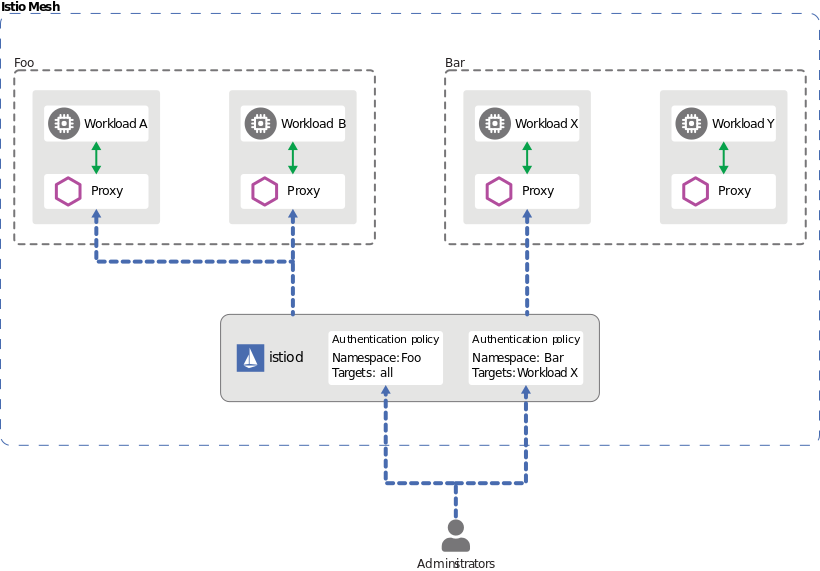
\includegraphics[width=0.9\textwidth]{chapters/images/chp2/arch-auth.png}
    \caption{Istio Security's v1.6 authentication architecture, from Istio Docs}
    \label{fig:autharc}
\end{figure}

\subsection{Identity}
In a traditional monolithic environment, identity was defined mostly by IP addresses or hostnames. For instance, we can recall the Apache HTTPD server rules, written using IPs.

In a distributed and microservices-oriented environment such as Kubernetes, due to its decoupled nature, the workload can be deployed on any machine, so IP addresses may change at any time. As it has been aforementioned, identity is either at origin or transport. At origin, the identity is defined as a subject (human) that is authenticated in various ways. However, at the transport layes, the old way of using IP is no longer possible due to the dynamic nature of the workload.

The \textit{Secure Production Identity Framework for Everyone} (SPIFFE)\footnote{See SPIFFE \href{https://spiffe.io/}{website}} specification is used to assign an identity to a workload, and it remains the same regardless of where it runs in a distributed environment. Istio has chosen a particular naming convention to provide an identity to a workload:


\begin{lstlisting}
  spiffe://cluster.local/ns/istio-lab/sa/productpage
           <cluster-name><ns><name-space><sa><service-account-name>
\end{lstlisting}

\noindent As it can be seen, the \texttt{spiffe} prefix is mandated by the SPIFFE specification (such as HTTP). Then, \texttt{cluster.local} is the name of a cluster (it should be different for different Kubernetes clusters if the intent is to use Istio to span multiple clusters using a single control plane). Then, \texttt{ns} is fixed, followed by \texttt{name-space}, where te workload is running. Finally, \texttt{sa} is fixed and \texttt{service-account-name} is the actual service account.

\textit{Citadel} is the implementation of the SPIFFE specification and is used to build a security solution in an untrusted network. Due to this, it is sometimes referred as security in a zero-trust network. Citadel issues SVID to the workload by signing the X.509 certificates upon a CSR being sent by a node agent running on every node on behalf of the Istio sidecar proxy running next to a workload. Once the proxy sidecar receives the certificate, it presents it to other workloads.

\section{Mutual TLS}
In order to secure service-to-service communication, it is tunneled from the client-side to the server-side via a sidecar proxy. Next, the inter-proxy communication is secured using mTLS. The benefit of mTLS is that the service identity is not expressed as a token bearer. It can be stolen, duplicated, or replayed from a source it hasn't been authenticated with. Istio's Citadel uses the concept of \textit{secure naming} and protection against attacks. The client-side verifies an authenticated service account and only allows the named service to run and pass through any network requests.

The mTLS feature can be used to validate client-level authentication by sending a certificate request message. This message will include the following:

\begin{itemize}
    \item It includes a list of distinguished root certificates that are tested by the server.
    \item The client responds to the server through a certificate message stating it is a distinguished name.
    \item The server verifies the client certificate.
    \item If the verification succeeds, the server has successfully authenticated the client.
\end{itemize}

This mTLS authentication is widely managed for business applications that have a limited number of homogeneous clients connecting to different web services. Overall, security requirements are higher priority when implementing mTLS versus any other consumer.

As it was already mentioned in \ref{chap:arch}, Istio has two modes that are implemented with mTLS: \textit{permissive} and \textit{strict}. The first one allows traffic in the HTTP and HTTPS protocols, whereas strict mode only allows traffic using the HTTPS protocol.

\subsection{Secure naming}
Securely naming services is an N-to-N mapping listed by server identities and detailed in certificates. All of the service names are defined by service discovery or DNS files. This mapping creates a list of service communications by authenticating an identity so that they can submit a client request for any service.

Secure naming is critical for multiple reasons, and the following scenarios will highlight the significance of having one:

\begin{itemize}
    \item A number of servers are running a service called \textit{Accounts}, and only the \textit{Payable} identity is allowed to authenticate these transactions.
    \item If a rogue user has access to the certificate and keys for another identity called \textit{Finance}, their objective is to inspect all of the traversed dta from the client, understand the service, and so on.
    \item The rogue user will set up and deploy an imposter server with the exact keys and certificates that have been detailed for \textit{Finance}.
    \item If the rogue user has hacked the DNS file or service discovery and mapped \textit{Accounts} to the imposter server.
\end{itemize}

If a new client calls the \textit{Accounts} service, with the forged server in place, the \textit{Finance} identity certificate is extracted. By using the secure naming information, \textit{Finance} will be checked if it is allowed to run the \textit{Accounts} service. The client will detect that this request is not allowed because only \textit{Payable} has been authenticated. Through this check, authentication will fails, and the rogue user will not be able to process their transaction.

This is a very critical step to securing communications within services because only service-specific identities that have been named within secure naming are allowed to initiate and receive requests. Without this process in place, rogue identity authentications such as man-in-the-middle attacks can hack the services, which can be detrimental to the reputation of a business.

\section{Policies}
One of the various rules that can be enforced by policies in Istio Security, is \textit{authentication}. 

In order to implement the authentication, the policy scope can be for an individual service, all of the services in a namespace, or all of the services in a service mesh. A rough idea of what happens using the Alpha API can be summarized in the following steps:

\begin{itemize}
    \item[1.] The policies are defined at the \textit{Citadel} level.
    \item[2.] \textit{Pilot} translates these policies to Envoy proxies to perform the required authentication mechanisms.
    \item[3.] \textit{Pilot} sends the configuration details, such as certificates and keys, to the Envoy proxy (PEP) asynchronously.
    \item[4.] As soon as the Proxy attached to a microservice receives the configuration, new authentication artifacts take effect. 
\end{itemize}

\textit{Origin} authentication is the responsibility of the client application and is used to acquire JWT and attach it to the request. JWT can be defined either for any request or for all of the requests except public paths, such as \texttt{/healtz} or \texttt{/status}, to expose them without authentication.

\textit{Transport} authentication is implemented through mTLS, and the destination rules defined by \textit{Pilot} determine which services in the mesh should initiate a TLS connection through the Envoy proxy.
For instance, it can be defined the policy for the \texttt{ns1} namespace for
\textbf{Service-D} in Citadel and Pilot pushes the mTLS policy to Service-D and 
the \texttt{ns1} namespace and leaves the other services intact. Similarly, two 
policies are defined for the \texttt{ns2} namespace. One is for 
\textbf{Service-A}, while the other is for all except Service-A. The 
\textbf{Target:All} policy is overridden by the one defined explicitly for 
Service-A.
This is known as policy enforcement (for authentication) at the namespace level.

Policies are stored by default in the \textit{root} namespace and apply to all workloads in the mesh. If they have a namespace scope, they are saved in the corresponding namespace. Moreover, if the \texttt{selector} field is specified, then the policy applies only on workloads in the namespace defined that match the defined selector. For what concerns the \texttt{kind}, there are two policies: \texttt{PeerAuthentication} and \texttt{RequestAuthentication}. The first one specifies the mTLS mode to enforce on target workloads, while the second one the values needed to validate a JWT (e.g. the issuer of the token, the location, the JWKS\footnote{From \href{https://auth0.com/docs/tokens/concepts/jwks}{Auth0 docs} "JSON Web Key Set (JWKS) is a set of keys which contains the public keys used to verify any JSON Web Token (JWT) issued by the authorization server and signed using the RS256 signing algorithm"}).

Authentication policies can be updated and, citing the documentation itself, " Istio pushes the new policies to the workloads almost in real time". This feature though, does not guarantee that the interested workloads receive the new policy at the same time. Indeed, some recommendations are available on Istio Docs in order to avoid problems during this phase of authentication policies update.

\section{In-depth analysis: permissive/strict modes}
As it has already been mentioned before, the Istio's mTLS \textit{permissive mode} can be used to enable both plain text and encrypted traffic on different services.

\noindent For instance, using the Beta API it can be defined a namespace-wide policy with the following \texttt{.yaml}:

\begin{lstlisting}
  apiVersion: "security.istio.io/v1beta1"
  kind: "PeerAuthentication"
  metadata:
    name: "default"
    namespace: "foo"
  spec:
    mtls:
      mode: STRICT
\end{lstlisting}

\noindent Where the mTLS mode is \texttt{STRICT} (so only encrypted traffic is permitted) and the namespace where it applies is \texttt{foo}. Istio allows the mode \texttt{PERMISSIVE} in order to facilitate the so called "onboarding" experience. For instance, an important use of this mode is during the migration of many non-Istio clients that communicate with a non-Istio server to Istio (that could be a challenging task for DevOps).

On one hand, this mode allows much more flexibility and simplicity on non-Istio service management. On the other hand, it drastically decreases the confidentiality by threatening the integrity of the exchanged messages between the parties. Plain text traffic could lead to really dangerous attacks that could break the entire cluster. A famous example is known as \textit{man-in-the-middle} (MITM) attack\footnote{Hijack attack, "[...] is an attack where the attacker secretly relays and possibly alters the communications between two parties who believe that they are directly communicating with each other.". Source: \href{https://en.wikipedia.org/wiki/Man-in-the-middle_attack}{Wikipedia.com}}.

Before the analysis of the real implementation of these two modes, it is really important to understand what are the default behaviours of the platform, because security must be integrated as part of the entire design process, including the definitions of the default configuration. More in details, from the documentation Istio states that "By default, Istio configures the destination workloads using PERMISSIVE mode." AAAAAA, but is this a good idea? The permissive mode is a general choice that can mislead the DevOps to think that \textit{everything} works out-of-the-box. Surprisingly, it does. The default mode is PERMISSIVE, but it is not set and left alone: Istio automatically enables mTLS traffic on pods that have proxies enabled and plain text traffic on pods without proxies. This is absolutely the best possible choice that joins security with ease of use. The default behaviour of the AuthN policy is set by using the Beta APIs through the \texttt{policy\_applier.go} in the \texttt{composePeerAuthentication()} function:
\vspace{0.3cm}
\begin{lstlisting}[title={\href{https://github.com/istio/istio/blob/ec8b8ba452b372b8ceaf8a5dea973bc561bf39b4/pilot/pkg/security/authn/v1beta1/policy\_applier.go\#L411}{GitHub permalink}}]
 outputPolicy := v1beta1.PeerAuthentication{
    Mtls: &v1beta1.PeerAuthentication_MutualTLS{
        Mode: v1beta1.PeerAuthentication_MutualTLS_PERMISSIVE,
    },
 }

\end{lstlisting}


The \textit{policy applier} script is part of the old \textit{Pilot Agent}, now merged with the old \textit{Node Agent} in an \textit{Istio Agent} available in each pods. Therefore, enforcing as default mode the \texttt{permissive} is the best possible choice.

\subsection{Protocol buffers}
In order to understand how the \texttt{.yaml} configuration file early mentioned in this section is converted into an effective authentication policy for mTLS (\textit{PeerAuthentication}), it first must be introduced the mechanism that Istio uses to serialize/deserialize data. In particular Istio defines component-level APIs and common configuration formats by using Google's \texttt{proto3}\footnote{Protocol buffers, a "[...] language-neutral, platform-neutral, extensible mechanism for serializing structured data – think XML, but smaller, faster, and simpler.". Source: \href{https://developers.google.com/protocol-buffers}{Google Dev}} to define the structure of each configuration file and then compile it with \texttt{protoc} in order to automatically generate the \texttt{.go} file with all the functions and variables able to serialize and deserialize, ready to be imported in other files as ready-to-use library. The \texttt{.proto} files are written in order to match each configuration file. For example, starting from a \texttt{.yaml} file:

\begin{lstlisting}
 # A custom resource that describes a Gateway resource
 apiVersion: networking.istio.io/v1alpha3
 kind: Gateway
 # ...
\end{lstlisting}

\noindent The corresponding \texttt{.proto} is:

\begin{lstlisting}
 package istio.networking.v1alpha3;
 message Gateway {
    // ...
 }
\end{lstlisting}

The \textit{PeerAuthentication}'s \texttt{proto3} definition is available in Istio's GitHub repository \textit{api}\footnote{\url{https://github.com/istio/api/blob/release-1.6/security/v1beta1/peer_authentication.proto}} alongside with the generated Golang and JSON code.

\subsection{Mutual TLS and secure naming implementation}
As mentioned in the introduction, Istio uses sidecars to deploy Envoy proxies that intercepts the inbound and outbound traffic from the workload applying encryption or not, based on the configuration loaded. This approach simplifies the implementation of the microservice because it does not depend on the used programming language and does not require libraries or extra software, since it intercepts and manages the packet itself. 
The certificate and private key of the proxy is provided by the \texttt{istio-agent}, that is responsible for the bootstrap of the sidecar itself, apart from the rotation of the secrets.

\begin{figure}
    \centering
    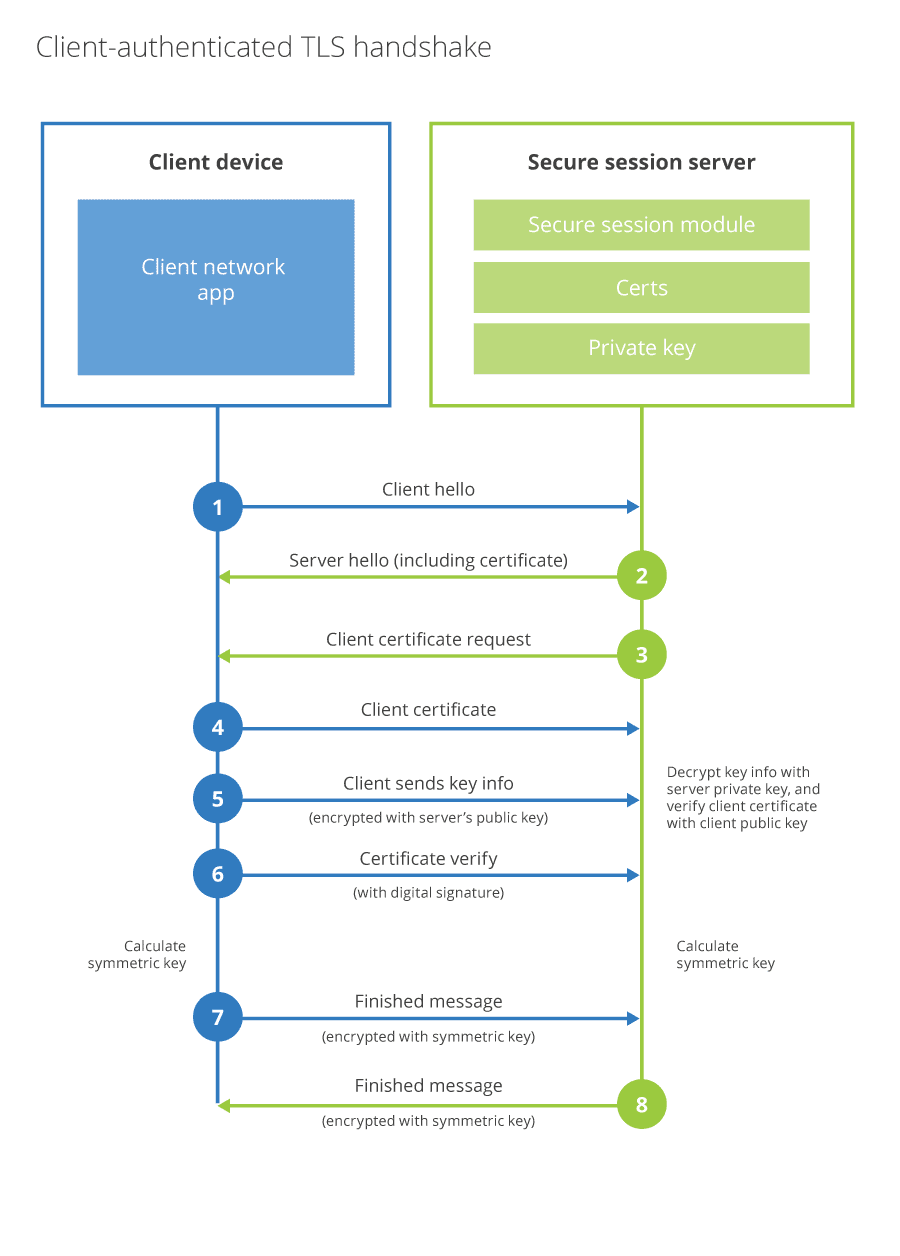
\includegraphics[width=0.5\textwidth]{chapters/images/chp2/mtls.png}
    \caption[Mutual TLS handshake]{Mutual TLS handshake\\Source: \url{https://developers.cloudflare.com/access/service-auth/mtls/}}
    \label{fig:mtls}
\end{figure}

In a standard scenario, the TLS handshake authenticates only the server. mTLS enables the authentication of the client too. Taking as example the Fig.~\ref{fig:mtls}, Istio's \texttt{PeerAuthentication} with the Envoy proxy enabled allows secure connection between two pods authenticating both the server and the client (microservices). In order to enforce the authentication policy, the interface \textit{PolicyApplier}\footnote{\url{https://github.com/istio/istio/blob/release-1.6/pilot/pkg/security/authn/policy\_applier.go}} provides essential functionalities to help configure Envoy:

\begin{lstlisting}
 type PolicyApplier interface {
    // InboundFilterChain returns inbound filter chain(s) for the given endpoint (aka workload) port to
    // enforce the underlying authentication policy.
    InboundFilterChain(endpointPort uint32, sdsUdsPath string, node *model.Proxy,
        listenerProtocol networking.ListenerProtocol) []networking.FilterChain

    // AuthNFilter returns the JWT HTTP filter to enforce the underlying authentication policy.
    // It may return nil, if no JWT validation is needed.
    JwtFilter() *http_conn.HttpFilter

    // AuthNFilter returns the (authn) HTTP filter to enforce the underlying authentication policy.
    // It may return nil, if no authentication is needed.
    AuthNFilter(proxyType model.NodeType, port uint32) *http_conn.HttpFilter
}
\end{lstlisting}


\noindent Each version of authentication policy will implement this interface.

In Istio, each workload is automatically assigned with an identity. Secure naming is a technology used in some mature companies such as Google. Its basic idea is to decouple the names / DNS names of the services from the identities that the services are running as. As an example, the service \texttt{frontend} (resolvable by \texttt{frontend} on DNS server) holds the certificate with identity \texttt{frontend-prod-team}. In Kubernetes, the identity \texttt{frontend-prod-team} is the service account of the workloads that are running the \texttt{frontend} service.

When doing mutual TLS handshake in Istio, the common practice of comparing the server's DNS name against the identities in the certificate (just like a browser verifies that the website presents a certificate with the identity \texttt{www.google.com} when someone is accessing www.google.com) is not correct. This is because the server side gives a certificate with its identity, not its service name. This requires the client to do a secure naming lookup during the handshake. The secure naming lookup asks this question: "Is the identity \texttt{frontend-prod-team} allowed to run the service \texttt{frontend}?" This operation is also called server authorization, as it corresponds to the client authorization done based on the client’s identity on the server side.
Secure naming offers the following benefits:

    \begin{itemize}
    \item It offers flexibility by decoupling the identity system from the service naming system. The service’s certificate does not need to be modified when a new DNS name is added or removed for the service.
    \item The certificate offers the identity of the server, instead of the service name the server is running for. This extra information can be useful for the internal traffic.
    \item It works well with the Kuberntes resource model. The Istio identity for a Kuberentes pod never changes (unless a trust domain migration happens).
    \end{itemize}

In Istio, the secure naming information is managed by Pilot. In Kubernetes clusters, Pilot has the information of: 

\begin{enumerate}
    \item Which pods are running each service.
    \item Which service account each pod is running as. 
\end{enumerate}

With these information, Pilot (integrated in \texttt{istiod}) constructs the secure naming information (i.e. which identities are running each service). The secure naming information is encoded in the \texttt{verify\_subject\_alt\_name} field in the CDS (Cluster Discovery Service) information and propagated to each Envoy sidecar.

mTLS and Secure Naming, combined with the secrets rotation implemented by \texttt{istio-agent} and with the default behaviours of the platform, guarantee a high level of security for what concerns the authentication and the encryption of the workloads, without giving away the ease-of-use for the basic tasks.  